\documentclass[11pt,a4paper]{article}
\usepackage[margin=0.8in]{geometry}
\usepackage{graphicx}
\usepackage{float}

\graphicspath{{../milestones/fcn3_collapsed_hmc/plots/onset_checks/}{../milestones/fcn3_collapsed_hmc/plots/locked_perp/}{../milestones/fcn3_collapsed_hmc/plots/ray/}}

\begin{document}

\begin{figure}[H]
  \centering
  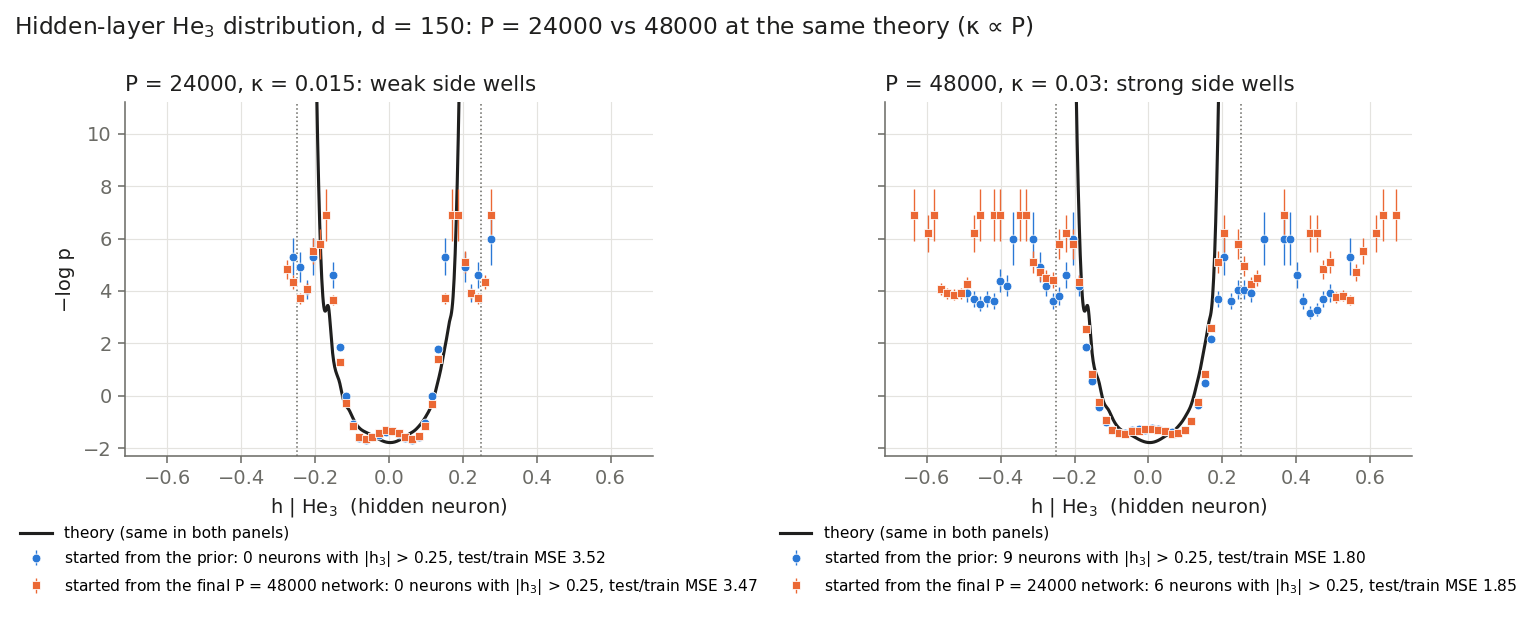
\includegraphics[width=\textwidth]{init_swap_he3_d150.png}
  \caption{Swapping the starting network between $P=24000$ and $P=48000$ at the same theory point. The He$_3$ side
  wells follow $P$, not the start, and they open where the network overfits less.}
\end{figure}

\begin{figure}[H]
  \centering
  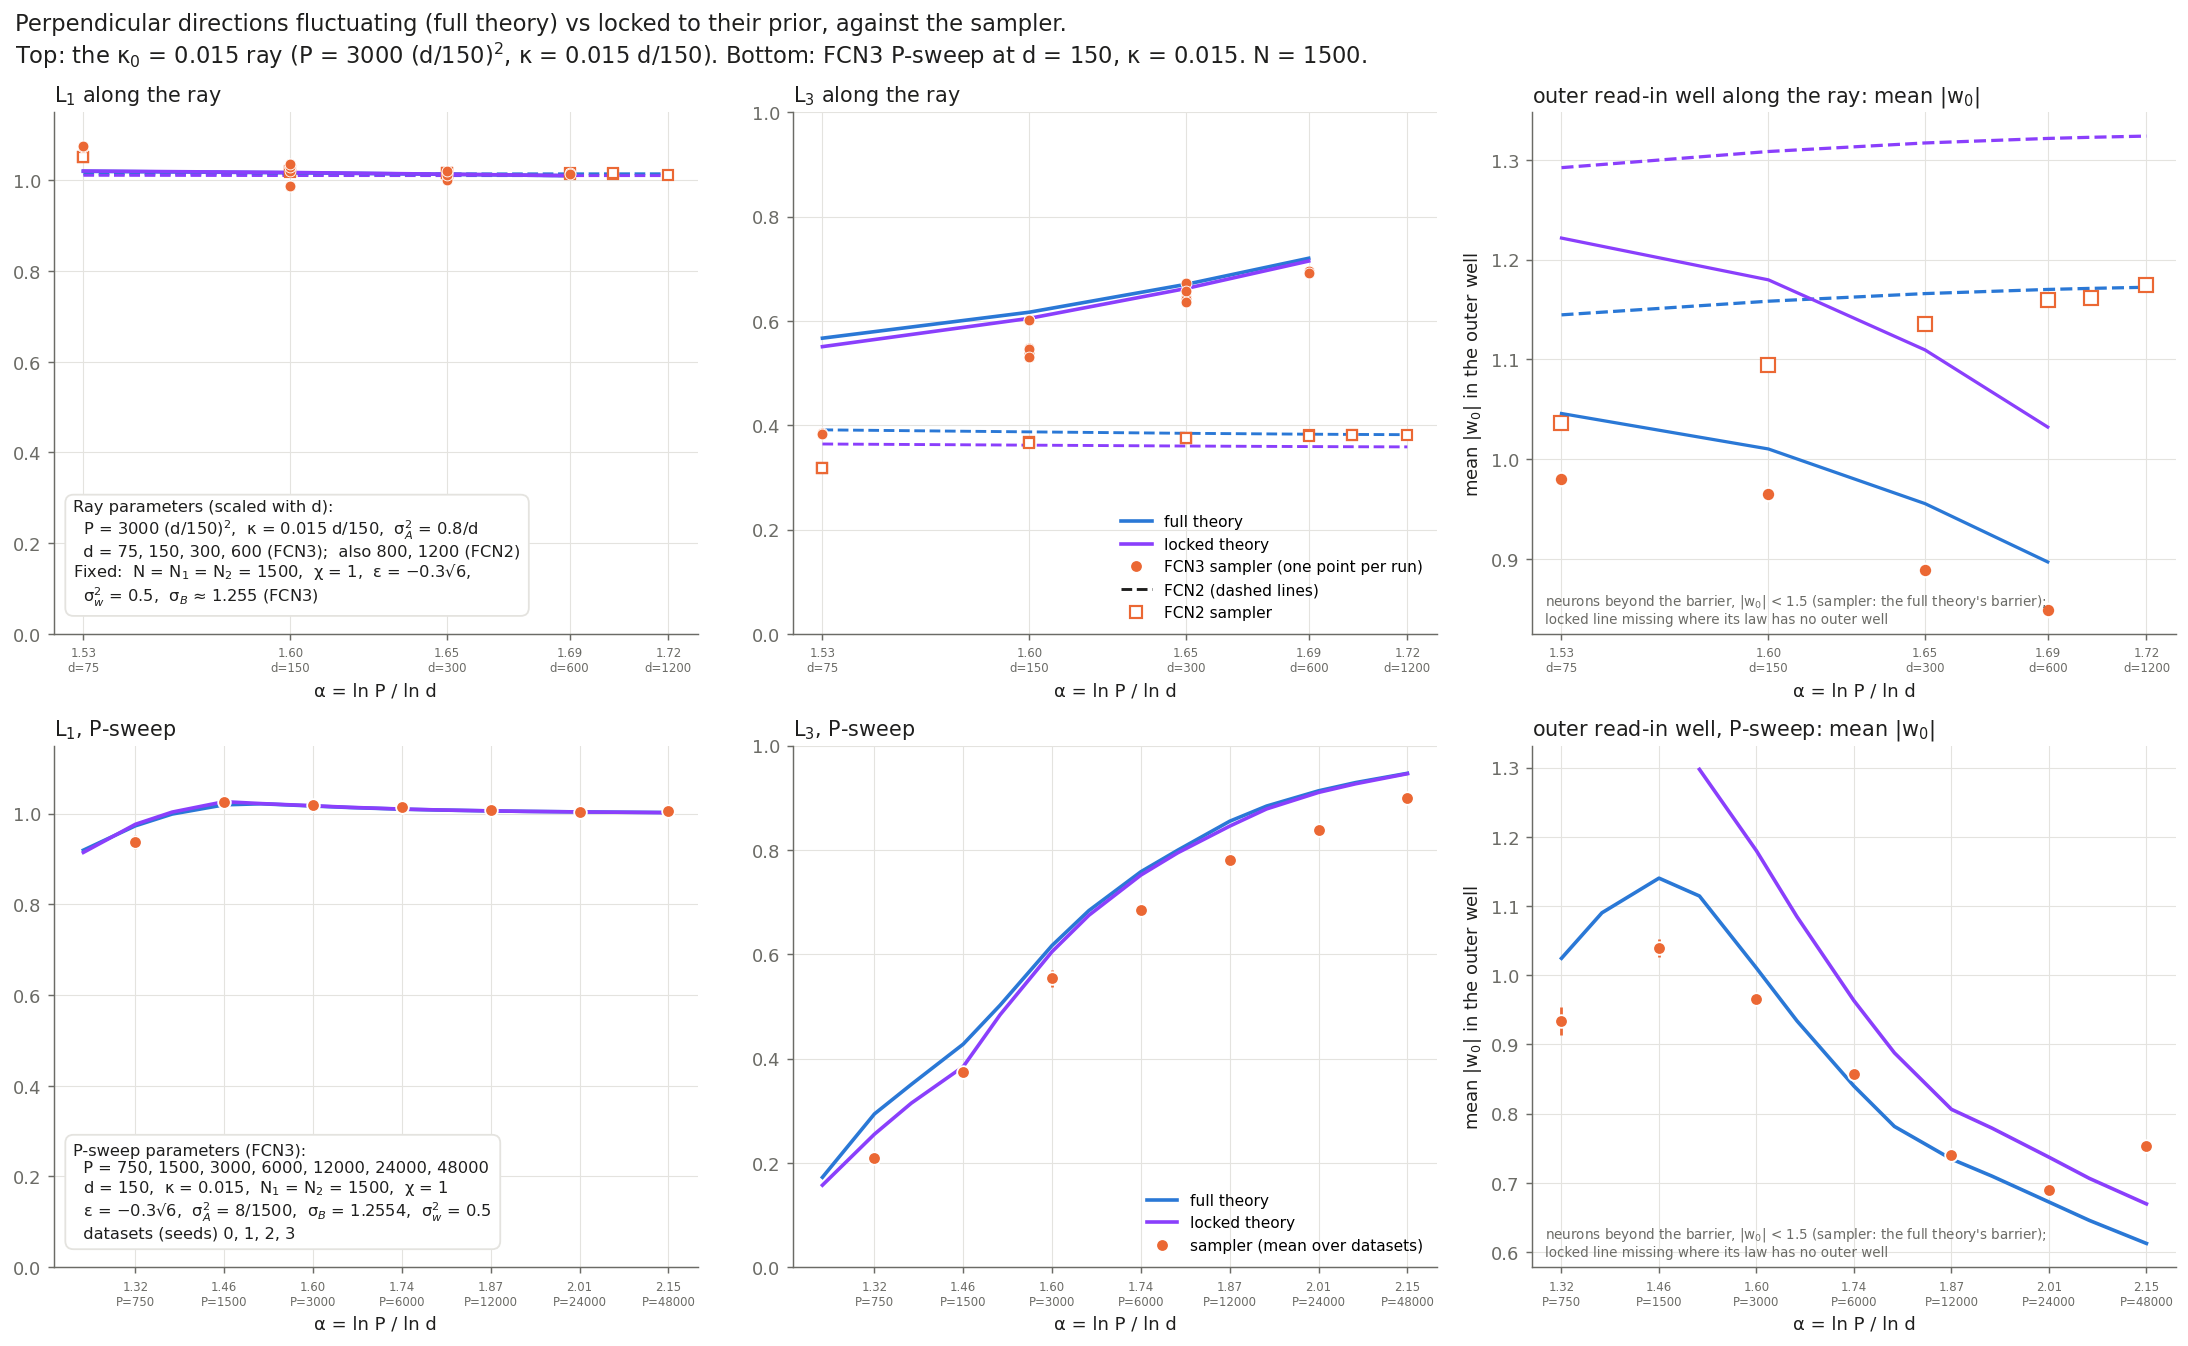
\includegraphics[width=\textwidth]{locked_perp_summary.png}
  \caption{Full theory against the theory with the perpendicular directions locked, on the ray (top) and the
  $P$-sweep (bottom).}
\end{figure}

\begin{figure}[H]
  \centering
  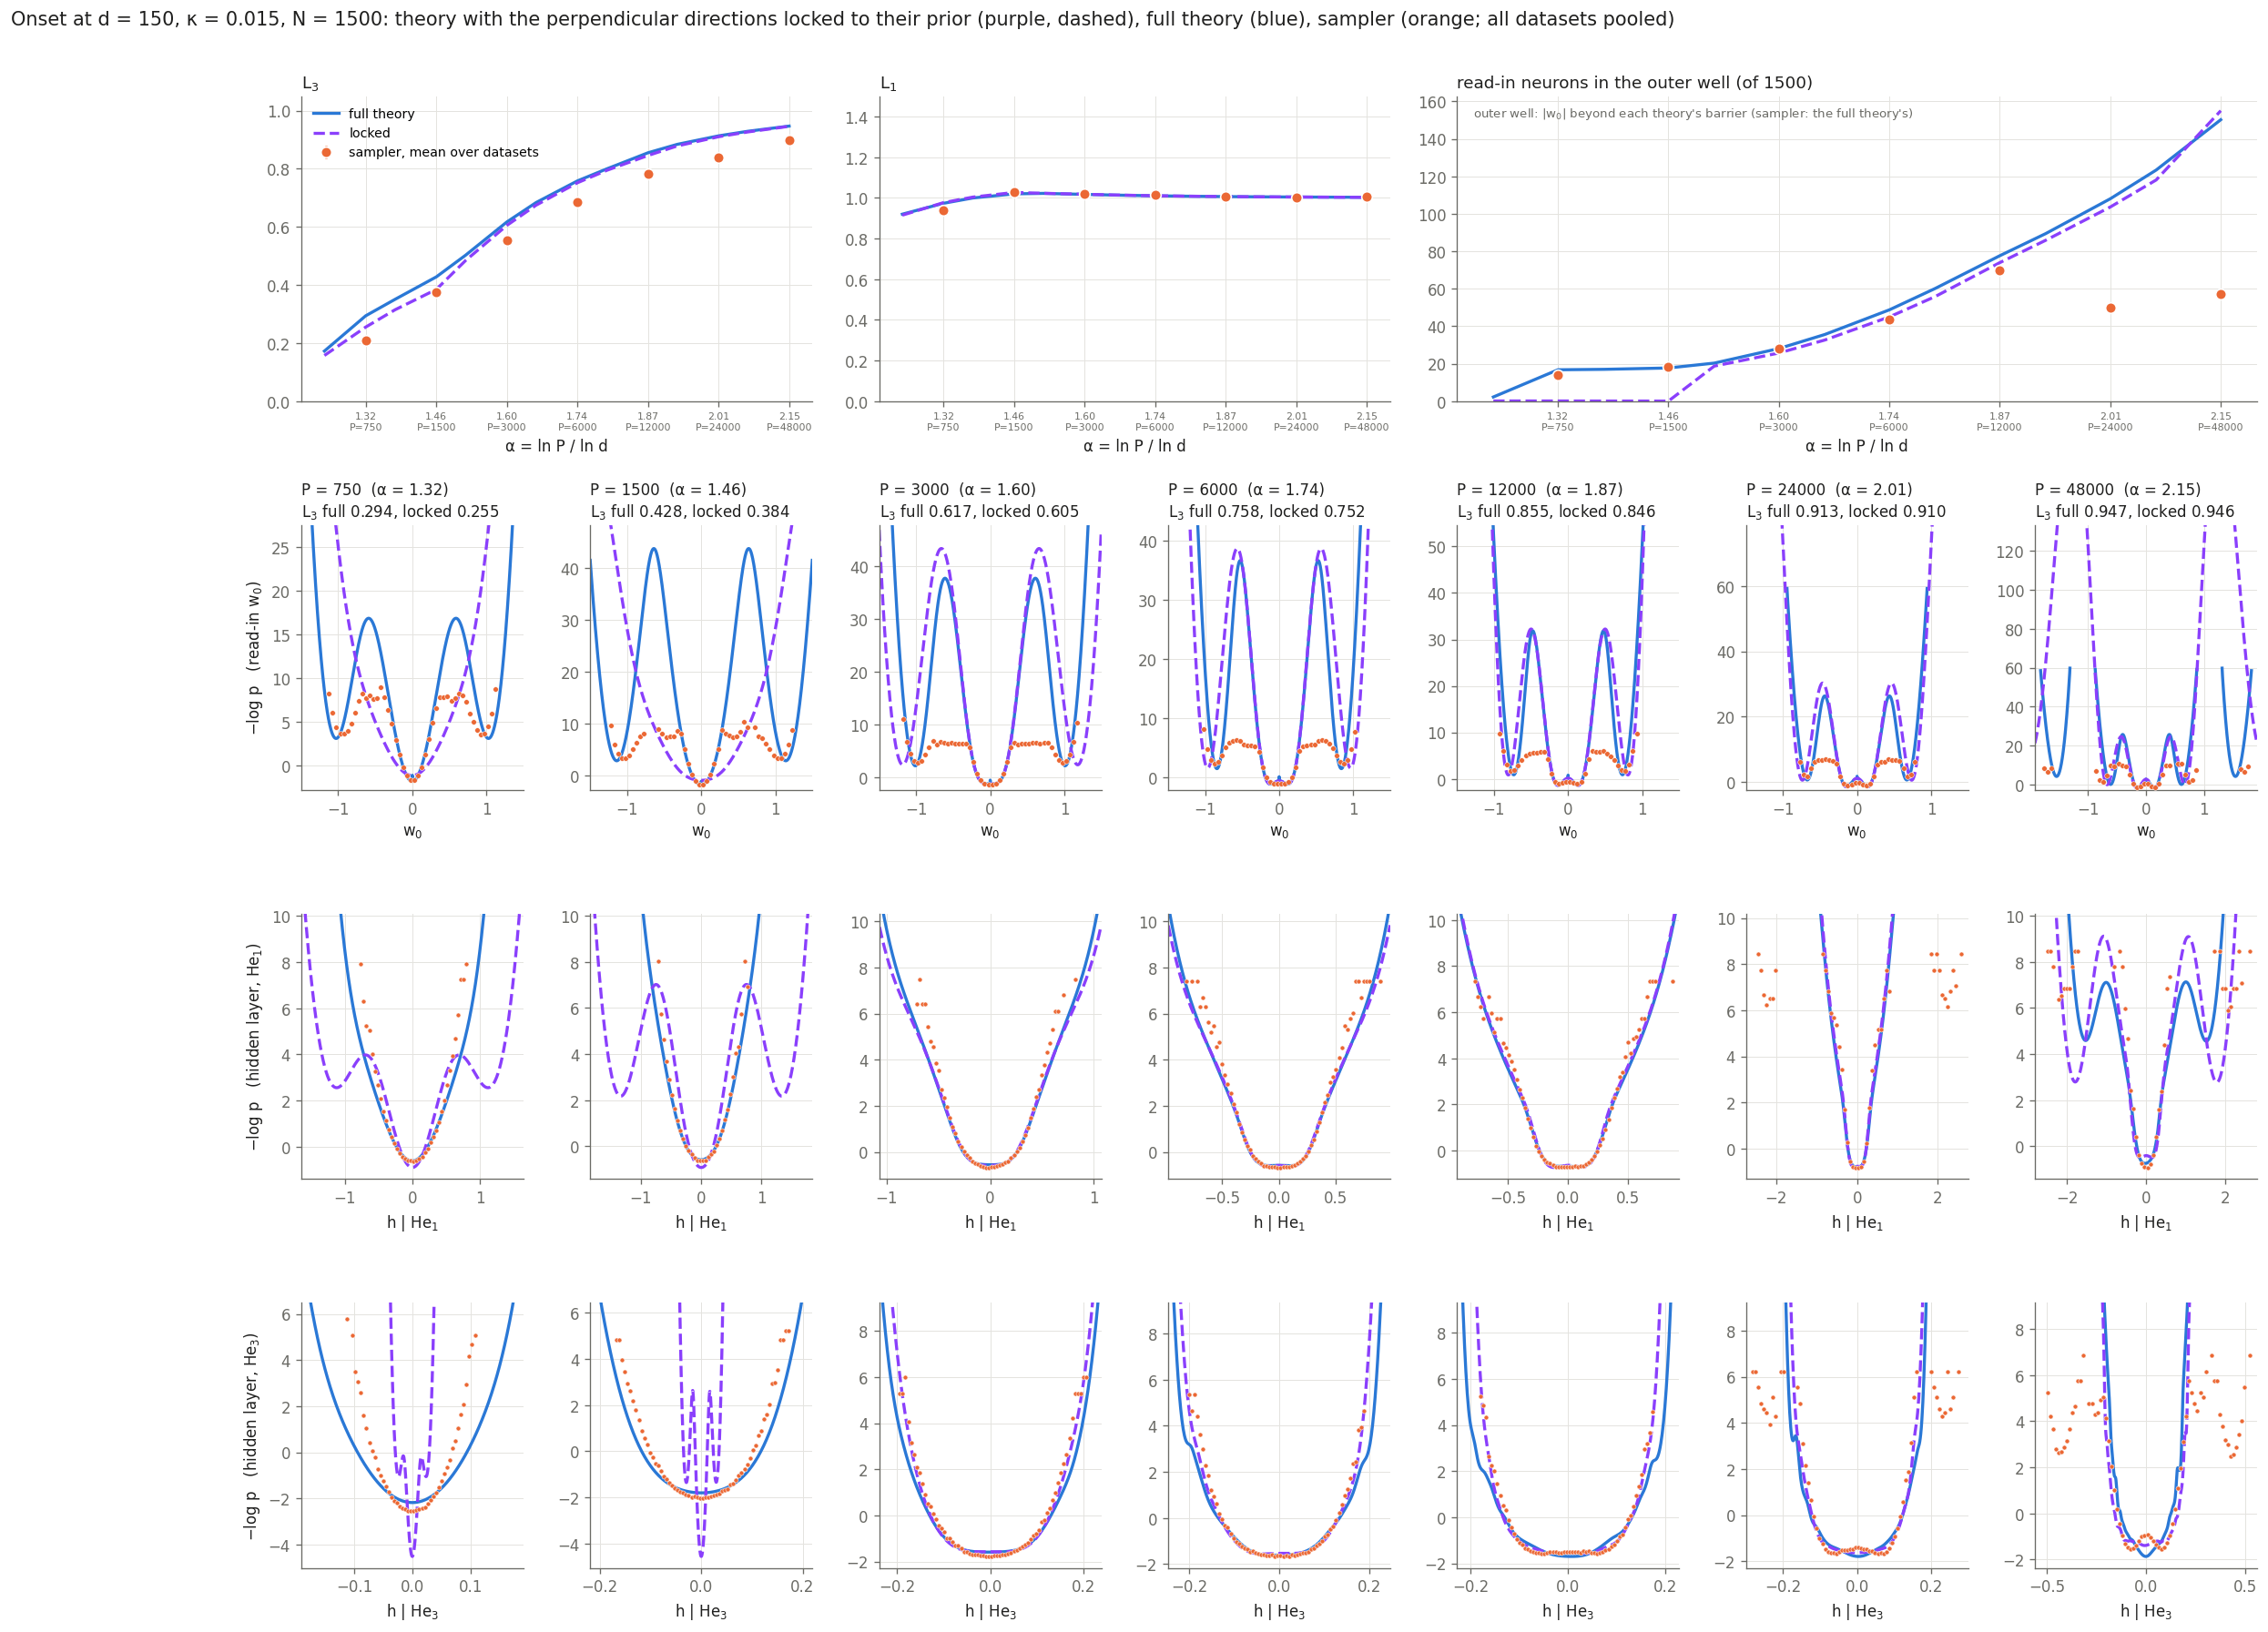
\includegraphics[width=\textwidth]{locked_perp_onset.png}
  \caption{Same comparison on the $P$-sweep, per $P$. The learnabilities barely move; the difference is in the actions
  of $w_0$, $h|\mathrm{He}_1$ and $h|\mathrm{He}_3$.}
\end{figure}

\begin{figure}[H]
  \centering
  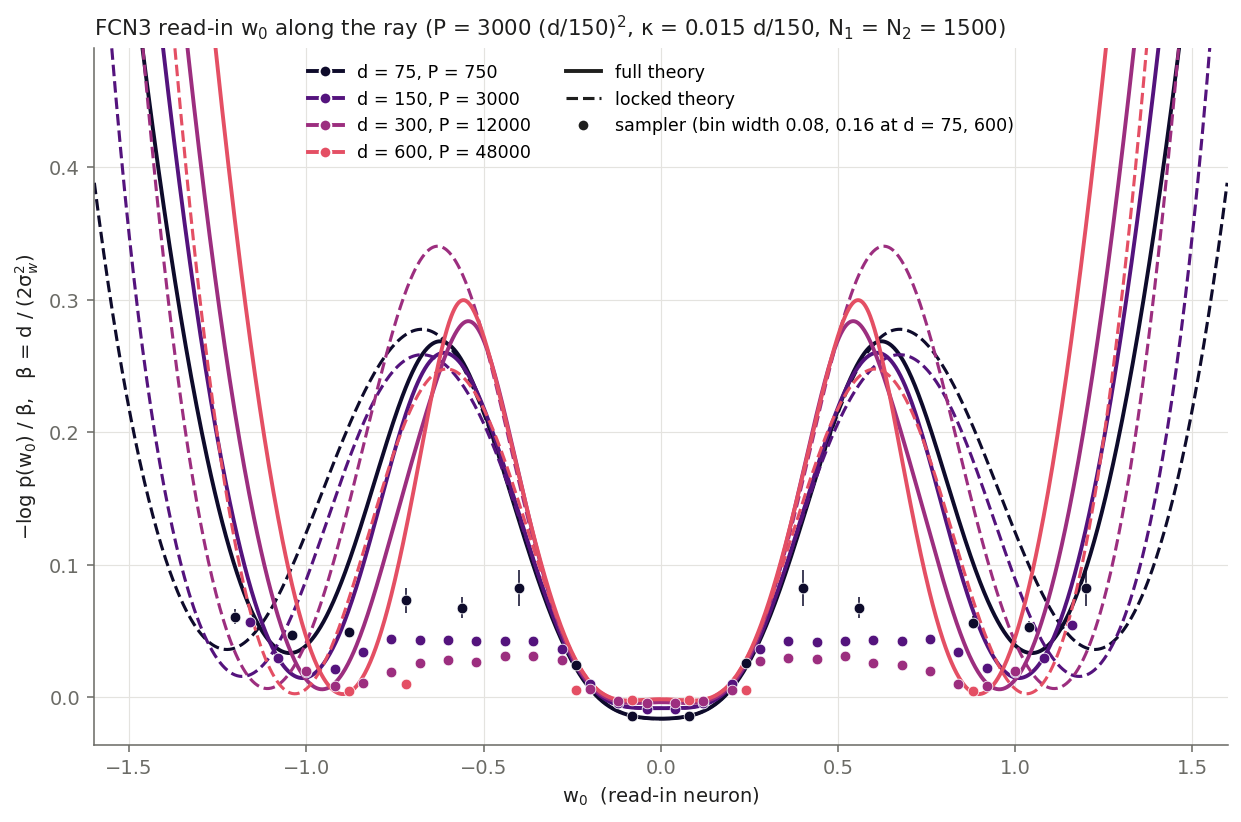
\includegraphics[width=\textwidth]{locked_perp_ray_fcn3_w0.png}
  \caption{FCN3 read-in $w_0$ along the ray, colour = $d$, divided by $\beta=d/2\sigma_w^2$ so all $d$ share one scale. Full and locked theory, sampler in wide bins.}
\end{figure}

\begin{figure}[H]
  \centering
  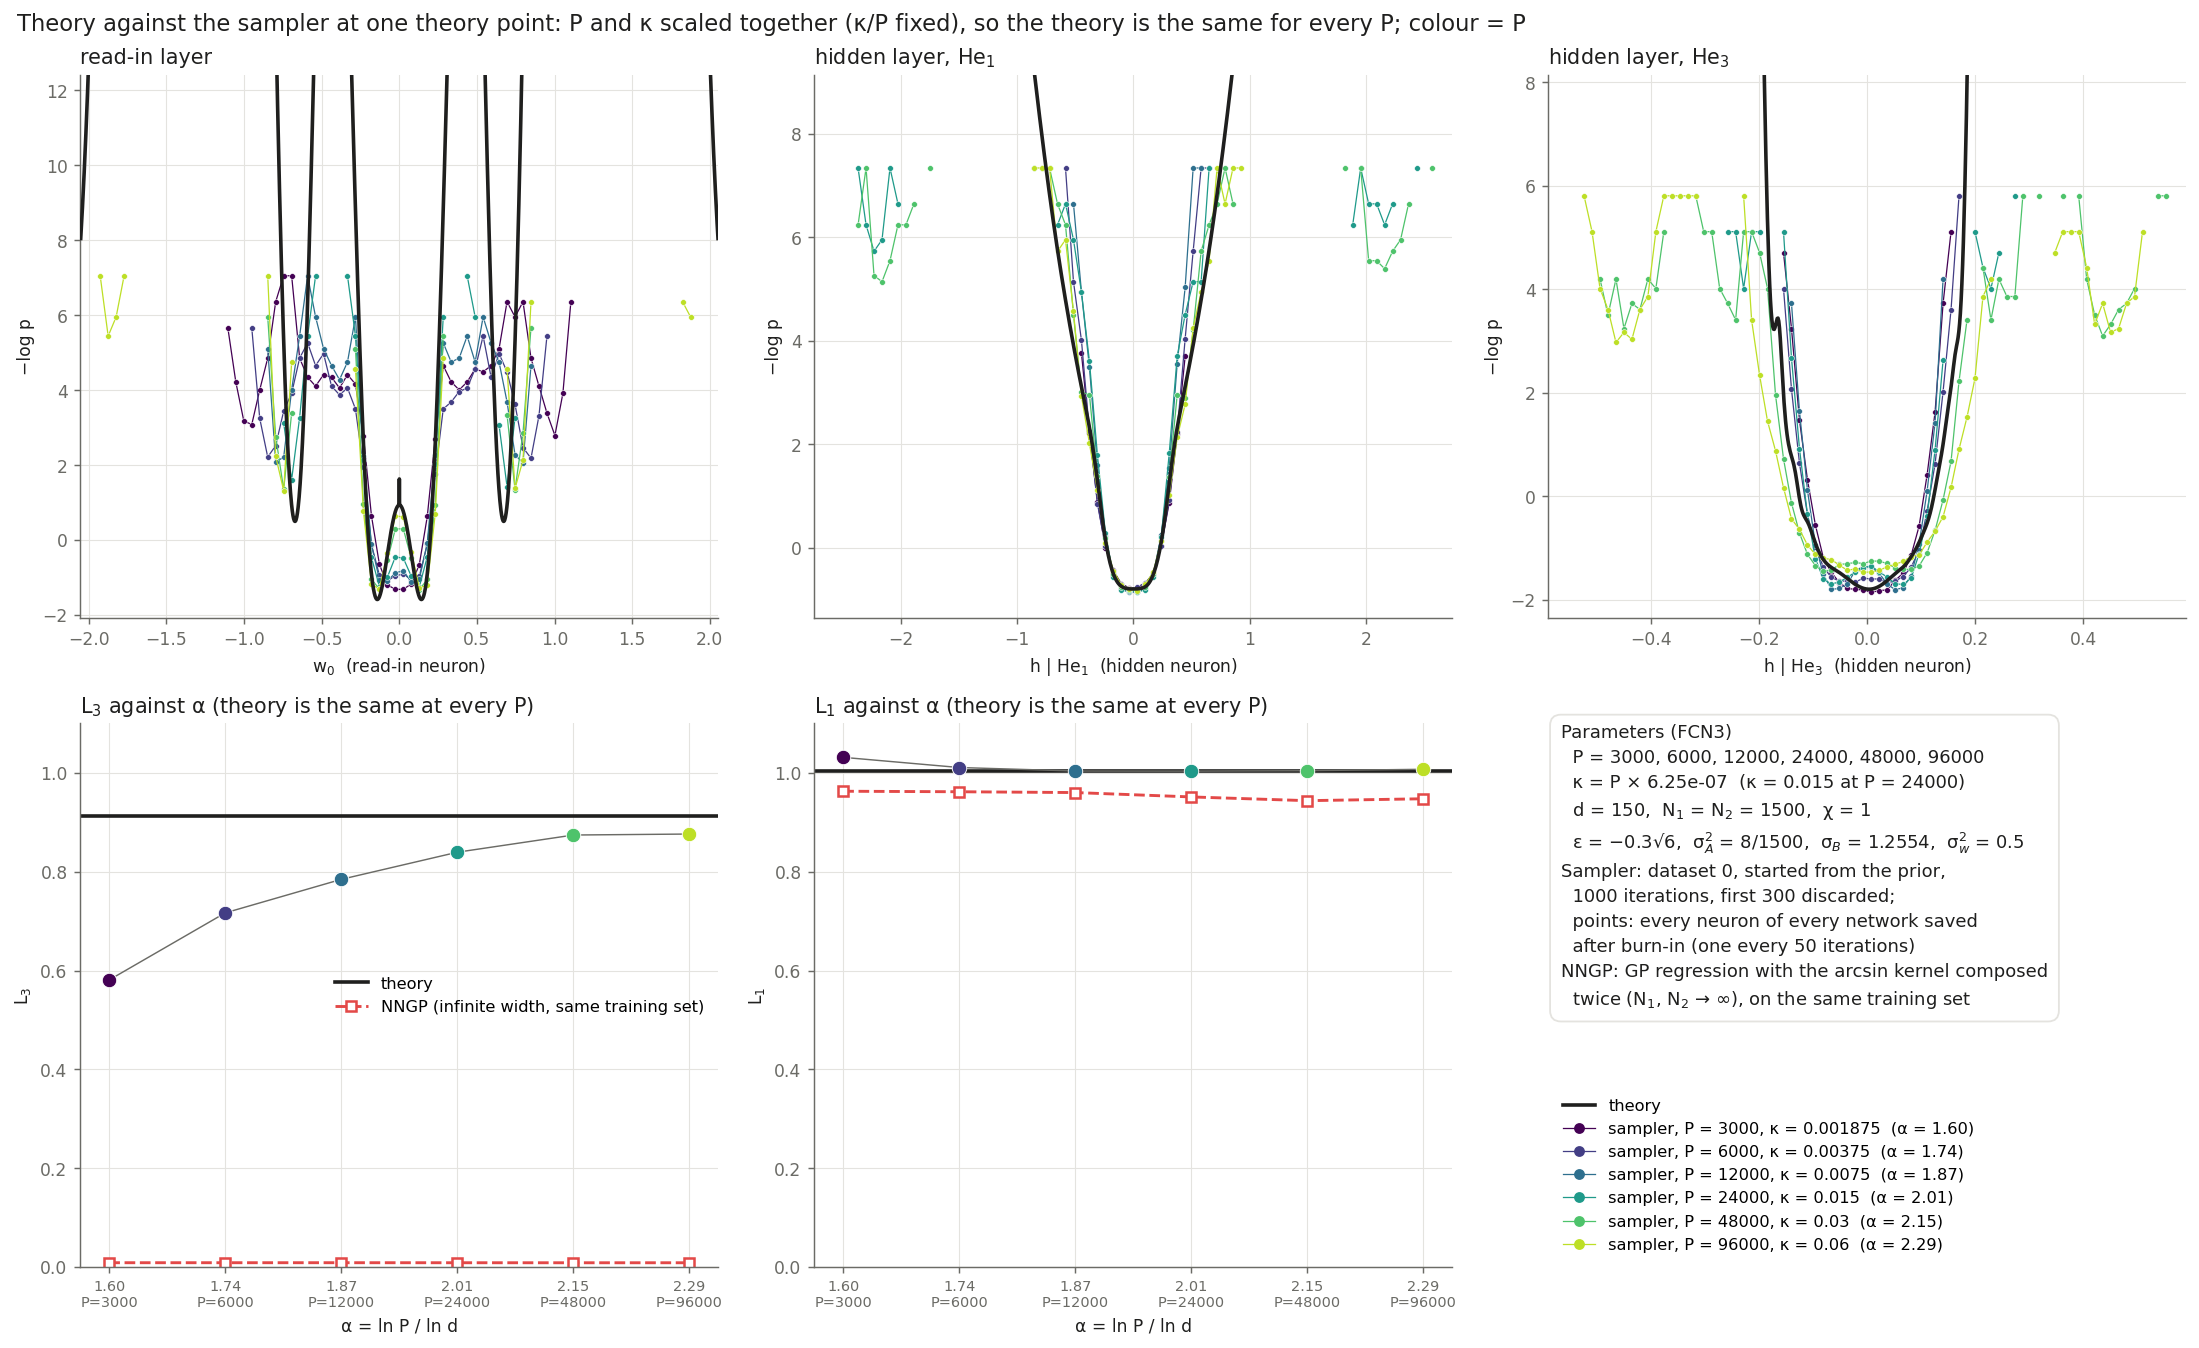
\includegraphics[width=\textwidth]{perp_compare_fixed_theory_d150.png}
  \caption{One theory point ($\kappa/P$ fixed), $P=3000$ to $96000$, with the NNGP.}
\end{figure}

\begin{figure}[H]
  \centering
  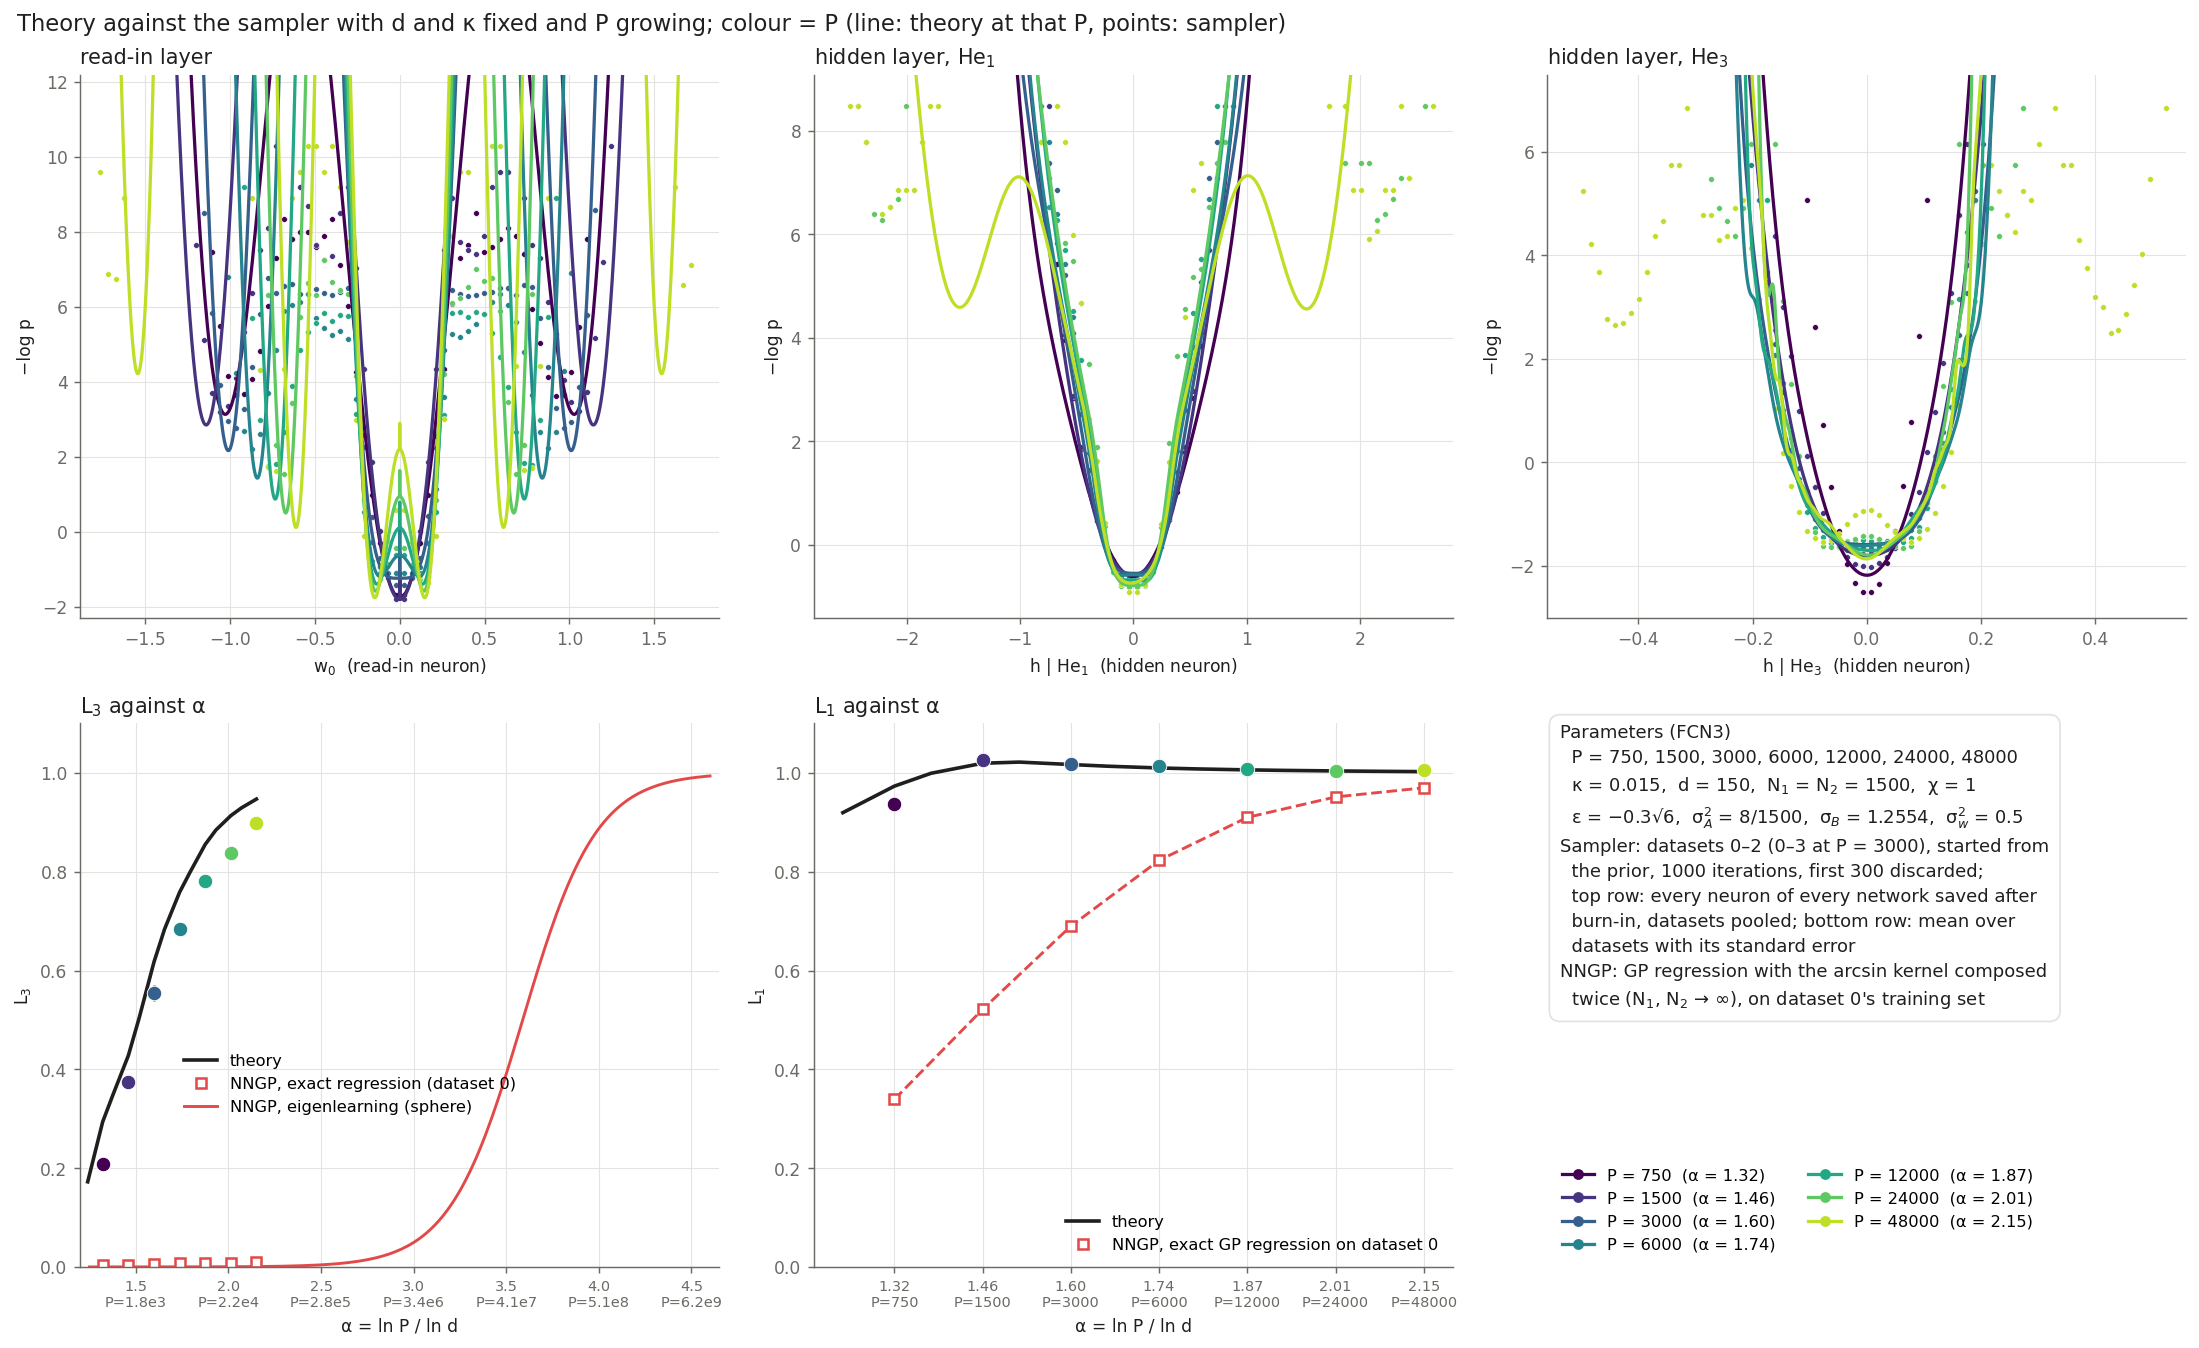
\includegraphics[width=\textwidth]{psweep_compare_d150.png}
  \caption{$P$-sweep at $d=150$, $\kappa=0.015$, with the NNGP. The NNGP only learns He$_3$ at $\alpha\approx 3.5$.}
\end{figure}

\begin{figure}[H]
  \centering
  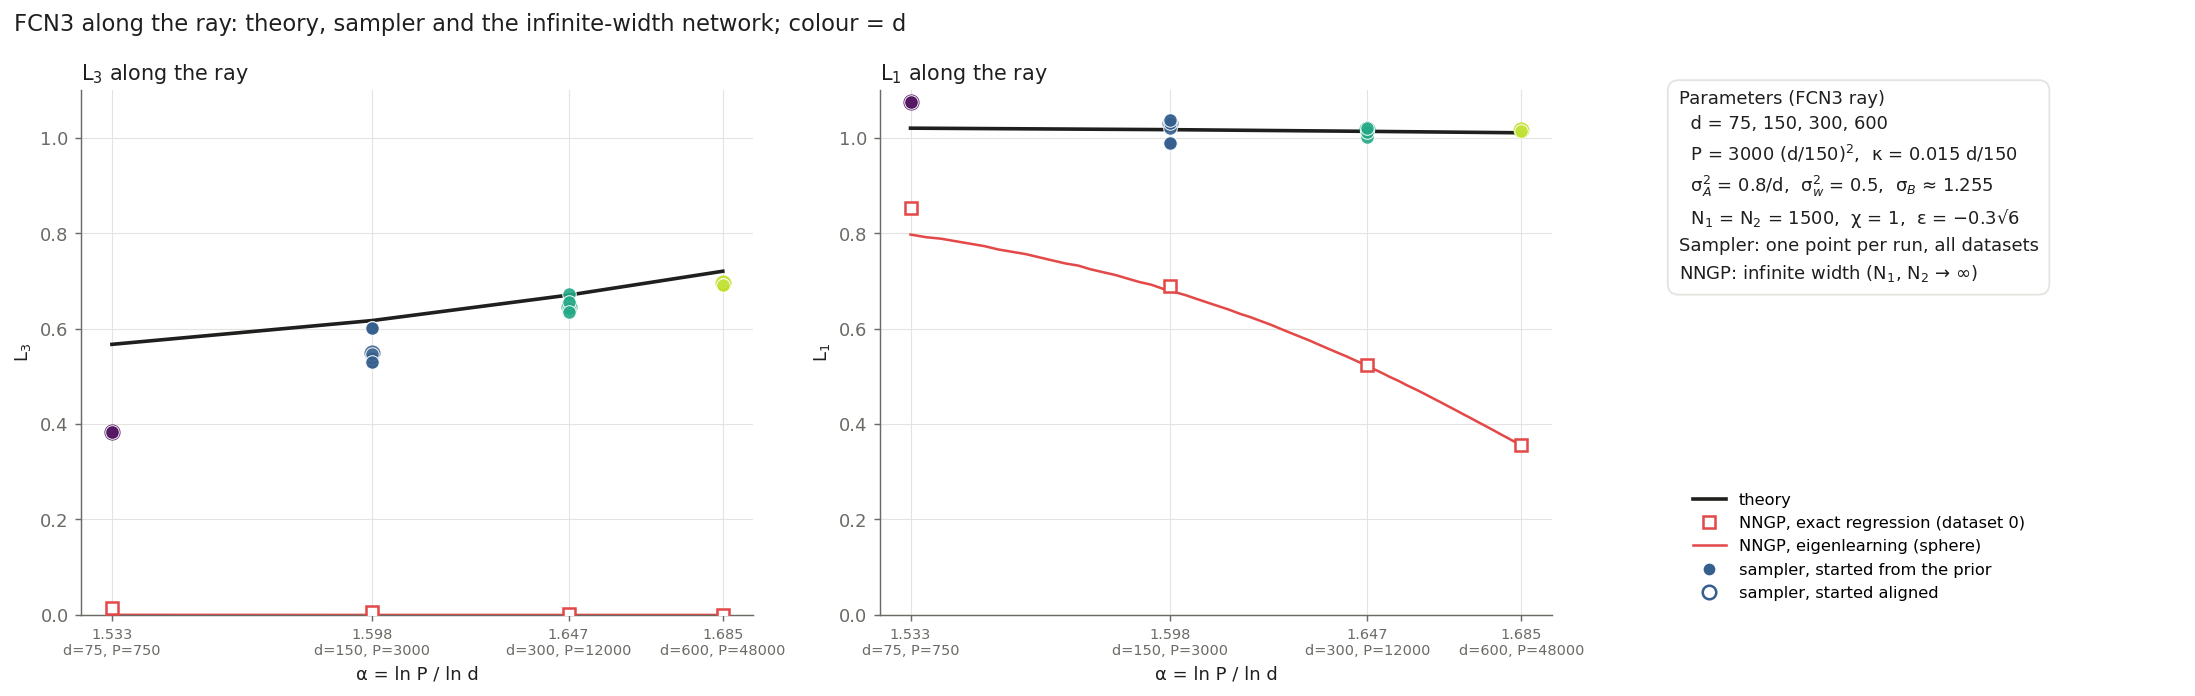
\includegraphics[width=\textwidth]{ray_learnability_fcn3.png}
  \caption{$L_3$ and $L_1$ along the FCN3 ray, with the NNGP.}
\end{figure}

\end{document}
